\chapter{Experiments}
\label{sq:experiments}

We tested the proposed methods on the developed dataset. Section \ref{sq:experimental_setup} summarizes the data processing and metrics. Section \ref{sq:results} presents and discusses the experimental results. Moreover, 
Section \ref{sq:training_pipeline} demonstrates 
efficient training pipelines for DQS,
and Section \ref{sq:ablation_study} reports the ablation study.

\section{Experimental Setup}
\label{sq:experimental_setup}

In our dataset, there are 2,758 question sets,
each of which is denoted by $\mathcal{Q}_U$ and was originally generated from the same outfit $O$. 
As explained earlier, we assumed that each question set $\mathcal{Q}_U$ is prepared for a user $U$
and the goal is to find the outfit $O$ that satisfies the user $U$,
by choosing effective questions from $\mathcal{Q}_U$.
In our experiments, we followed the same experimental protocol 
as that used in the analysis of the developed dataset.
For every question pair ($Q_1$, $Q_3$) in a question set $\mathcal{Q}_U$, we assumed a situation where $Q_1$ had been already asked and answered. 
The task is to find a question $Q_2$ from the rest of the questions in 
$\mathcal{Q}_U$.
The performance of the question selection is measured by 
the accuracy of the best question selection,
and the recommendation performance after the question selection.
The accuracy is defined as the fraction of cases where the question selection algorithm can identify the best question, as was defined in Section \ref{sq:analysis}.
The success of the recommendation was measured by nDCG,
an effectiveness measure for rankings,
where the grade is 1 for a relevant outfit and 0 for the others. 

% In each question set, there are multiple questions generated from the same outfit. Each question contains 5 item IDs. Our experimental goal is to let the model choose the best question from a list of candidates. When the model has chosen a good question, it should move the recommendation of answer prediction to the next question. As a result, we use the recommendation result from the next question to determine whether or not the selection is good In summary, we use the outcome of the third question recommendation to assess the quality of the second question, which is chosen based on the first question and the user's response.

% Thus, in each round of training, we need two questions and multiple selectable questions. To achieve a subset that fit our training needs, we applied an algorithm to the generated dataset. For a question set with $n_Q$ questions, the algorithm selects two of them and treats them as the first and third questions. The rest of the questions are thought to be selectable. We only use question sets with more than six questions to generate a subset to improve model robustness. Following that, we apply the bidirectional LSTMs model to the first and third questions to evaluate these selectable questions.



% We used the following metrics as effectiveness measures: 1) the accuracy of choosing the best question, 2) nDCG@1 of , and 3) nDCG@5 of question score ranking. The accuracy is only counted if the model selects the same question with ground truth. nDCG provides more extra information on the error between model and truths.

The LTR model was implemented in XGBoost~\cite{chen2016xgboost}. 
The DQS models were trained by the Adam optimizer~\cite{kingma2014adam}. 
% 学習データについて
We split the dataset to a training set and a testing set with a 3:1 ratio. 
To prevent leakage, it was guaranteed that all the question sets generated from the same outfit were in either the training set or the testing set.
Each model was trained only with the train set, 
while the evaluation ran onto the test set.

%%%


\section{Results}
\label{sq:results}

\begin{table}[t]
\caption{The performance of the proposed methods.}
\centering
\begin{tabular}{lccc}
\toprule
              & Accuracy             & nDCG@1          & nDCG@5          \\ 
\midrule
Random        & 0.171          & 0.500          & 0.717          \\
LTR    & 0.220          & 0.596          & 0.782 \\
\texttt{DQS-share-200} & \textbf{0.414} & \textbf{0.710} & \textbf{0.822}          \\
\texttt{DQS-ind-200}   & 0.392          & 0.701          & 0.814          \\ 
\bottomrule
\end{tabular}
\label{normal-train-results}
\end{table}

Table \ref{normal-train-results} shows the effectiveness of the question selection models, which include the simplest baseline that selects questions randomly (Random).
The proposed models, \texttt{DQS-*}, were trained for 200 epochs in this experimental setting. 
The results show that our DQS models outperformed not only 
the random baseline but also the LTR model, to a large extent. 
Notably, \texttt{DQS-share-200} achieves the 41.44\% accuracy of best question prediction. \texttt{DQS-ind-200}, which does not share parameters in two Set Transformer models, did not show a better performance than \texttt{DQS-share-200}. A two-way ANOVA of nDCG@5 revealed that the system effect is statistically significant ($F(3, 24,960) = 1329.458, p < 0.05$). 
A Tukey's HSD test shows that all the differences except for
that of \texttt{DQS-share-200} and \texttt{DQS-ind-200} are statistically significant ($p < 0.05$). 
% The effect sizes of these pairs are 0.547, 0.883, 0.808, 0.336 and 0.261 for Random-LambdaMART, Random-\texttt{DQS-share-200}, Random-\texttt{DQS-ind-200}, LambdaMART-\texttt{DQS-share-200}, and LambdaMART-\texttt{DQS-ind-200}, respectively.

\begin{figure}
  \centering
  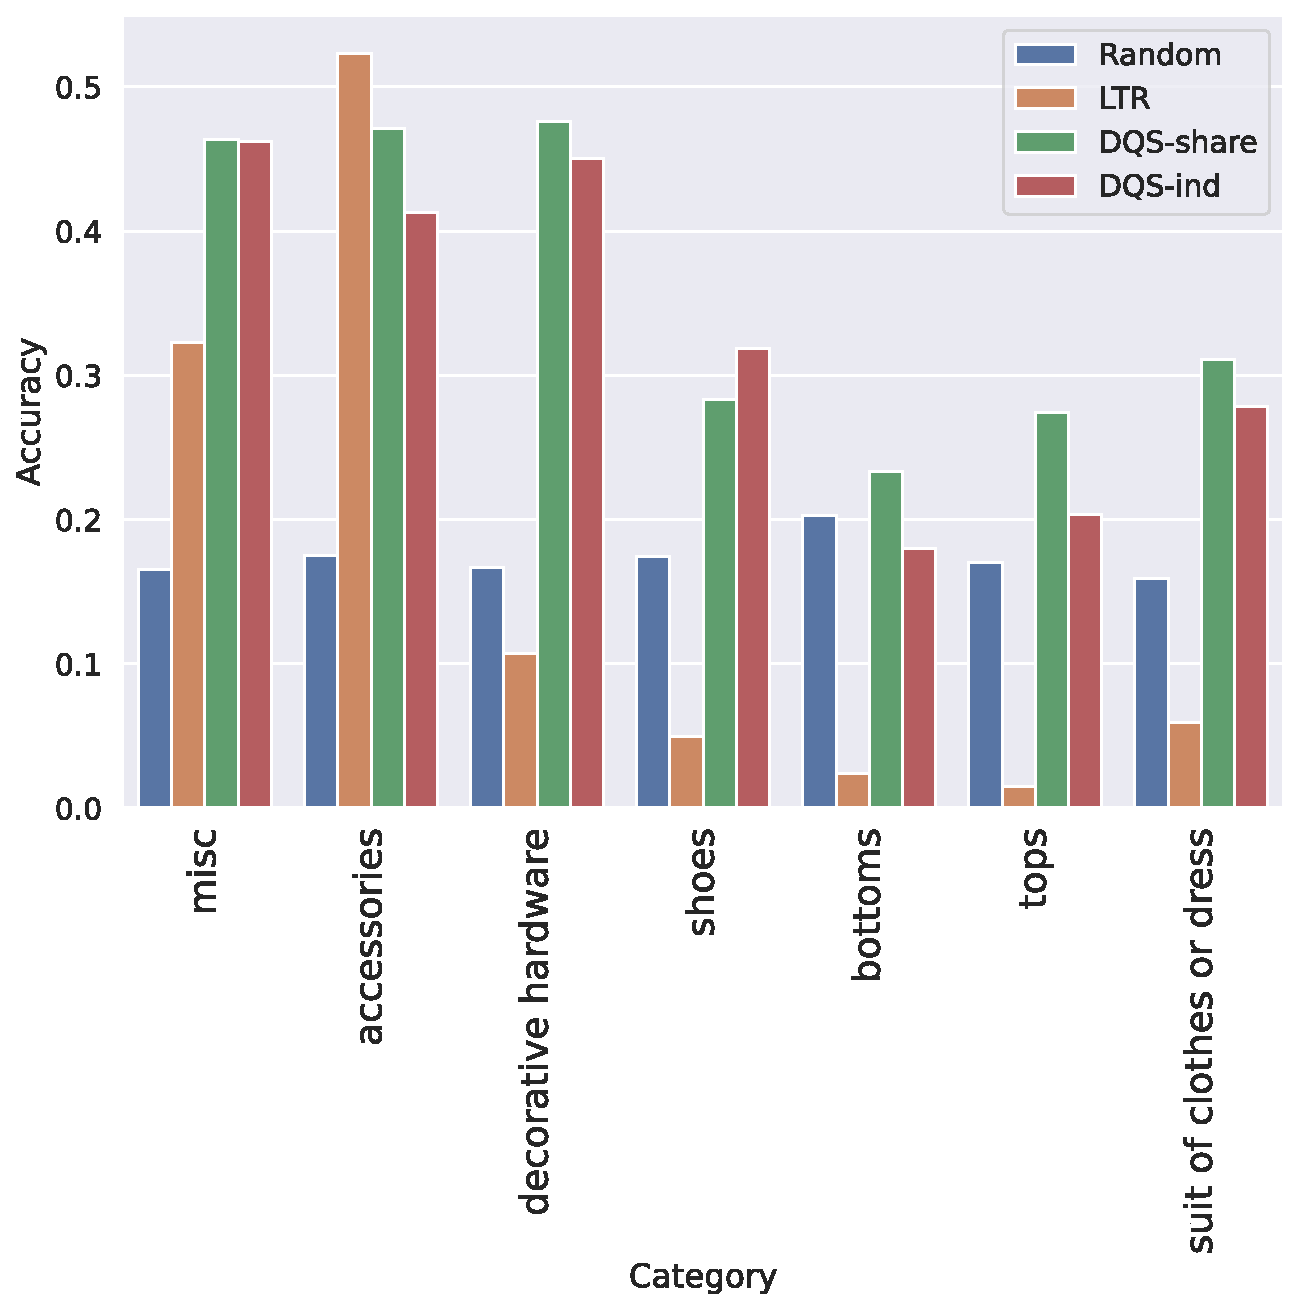
\includegraphics[width=0.6\linewidth]{figures/category_acc.pdf}
  \caption{Accuracy of the proposed models in different categories.}
  \label{category-acc}
%   \vspace{-1em}
\end{figure}

\begin{figure*}
  \centering
  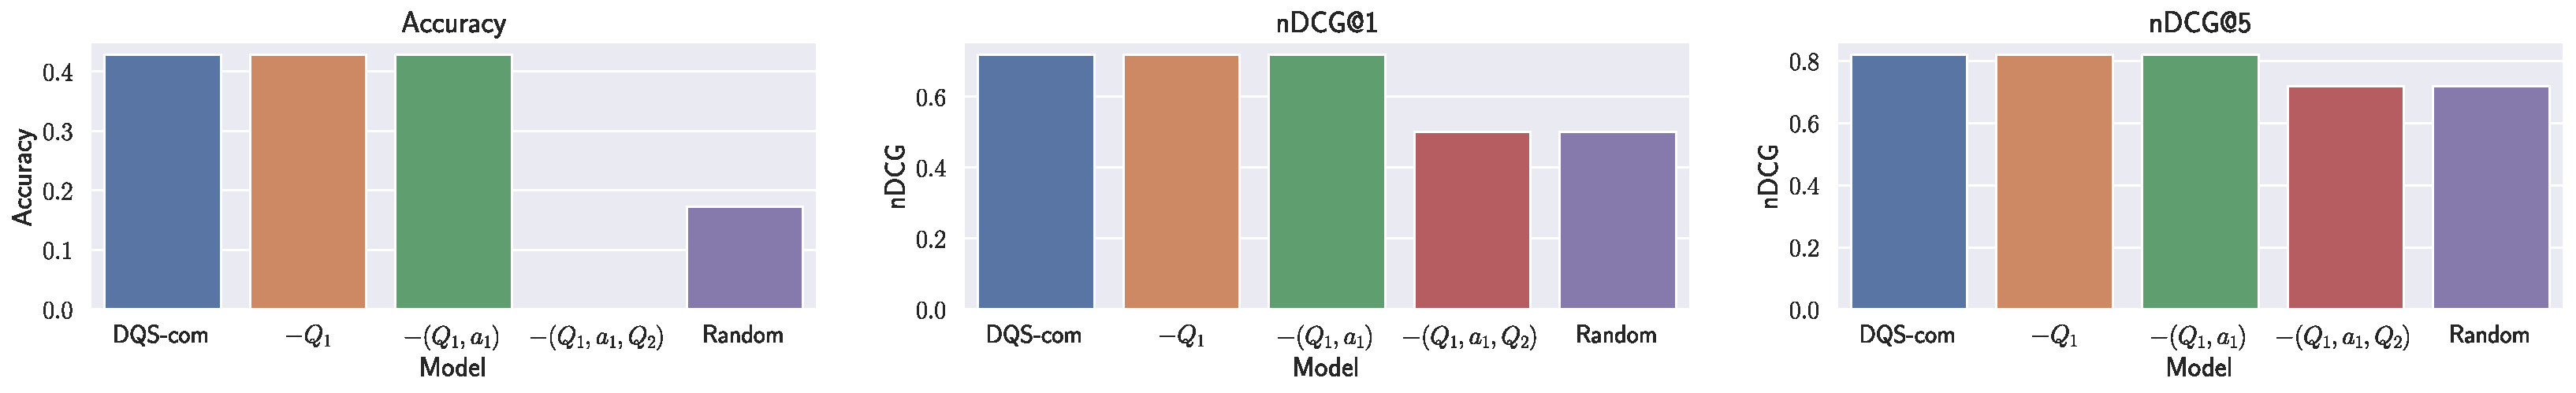
\includegraphics[width=\linewidth]{figures/ablation.pdf}
  \caption{Accuracy, nDCG@1, and nDCG@5 of the ablations of $Q_1$, $(Q_1, a_1)$, and $(Q_1, a_1, Q_2)$.}
  \label{ablation}
%   \vspace{-1em}  
\end{figure*}

Figure \ref{category-acc} reports the accuracy of proposed models in different categories. 
While LTR, \texttt{DQS-share} and \texttt{DQS-ind} all achieved substantial improvements over the random baseline, 
there exist significant differences across categories.
The LTR model outperformed in the accessories type question. However, it cannot handle bottoms and tops; the accuracy is even worse than the random baseline. 
This is probably because the LTR model highly relies on the category information and is likely to select questions in the accessories category.
On the other hand, DQS shows its superiority across all the categories against the other methods.


\section{Training Pipeline}
\label{sq:training_pipeline}


Furthermore, we propose a practical training pipeline for the DQS models. 
As shown in the following experimental results, it turned out that the training of Set Transformer is a bottleneck of efficient training. 
Thus, we aimed to reduce the training time of Set Transformer models without loss of model performances. 
The idea came from transfer learning~\cite{pan2009survey}:
we first pre-train Set Transformer so that its output for a question $Q$
becomes close to the mean of item embeddings in $Q$.
More precisely, we trained ${\rm ST}$ to minimize the mean absolute error,
$\| {\rm ST}(Q) - \frac{1}{|Q|}\sum_{i \in Q} {\mathbf i} \|$,
for each training question $Q$.
A DQS model then loaded the trained parameters of the Set Transformer and started the learning of the full model. 
Additionally, to verify the effectiveness of the mean item embedding, 
we introduced a new model \texttt{DQS-mean}
in which Set Transformer in DQS is replaced with a mean aggregator. 
In the following experiments, we pre-trained {\rm ST} for 100 epochs with the Adam optimizer.


\begin{table}[t]
\caption{The performance of DQS models with the special training pipelines.}
\centering
\begin{tabular}{lccc}
\toprule
                              & Accuracy             & nDCG@1          & nDCG@5          \\ 
\midrule
Random                        & 0.1710          & 0.5002          & 0.7173  \\
LTR                    & 0.2202          & 0.5957          & 0.7824 \\
\texttt{DQS-mean-200}                  & 0.3089          & 0.6691          & 0.8053          \\
\texttt{DQS-share-200}                 & 0.4144          & 0.7102          & \textbf{0.8224}          \\
\texttt{DQS-ind-200}                   & 0.3917          & 0.7010          & 0.8135          \\
\midrule
\texttt{DQS-share-50-sp}     & 0.4123          & 0.7077          & 0.8140          \\
\texttt{DQS-share-100-sp}    & 0.4269          & 0.7187          & 0.8199          \\
\texttt{DQS-ind-50-sp}       & 0.3961          & 0.7118          & 0.8179          \\
\texttt{DQS-ind-100-sp}      & 0.4117          & 0.7072          & 0.8187          \\
\texttt{DQS-com-100-sp}  & \textbf{0.4282} & \textbf{0.7190} & 0.8206          \\ 
\bottomrule
\end{tabular}
\label{special-train-results}
\end{table}

\begin{table}[t]
\caption{Training time of DQS models with the special training pipelines.}
\centering
\begin{tabular}{lcr}
\hline
                            & \# Epoch & \multicolumn{1}{c}{Time} \\ \hline
Set Transformer pre-training & 100      & 53mins                   \\
\midrule
LTR                  & 200       & 2mins                  \\
\texttt{DQS-mean-200}                & 200      & 1hr 37mins               \\
\texttt{DQS-share-200}               & 200      & 1d 5hrs 45mins          \\
\texttt{DQS-ind-200}                 & 200      & 1d 15hrs 38mins          \\
\midrule
\texttt{DQS-share-50-sp}             & 150      & 8hrs 5mins              \\
\texttt{DQS-share-100-sp}            & 200      & 15hrs  35mins            \\
\texttt{DQS-ind-50-sp}               & 150      & 10hrs 29mins             \\
\texttt{DQS-ind-100-sp}              & 200      & 19hrs  56mins            \\
\texttt{DQS-com-100-sp}              & 200      & 17hrs 10mins             \\ \hline
\end{tabular}
\label{cost-time}
\end{table}

Table \ref{special-train-results} reports the performance of DQS models,
and Table \ref{cost-time} shows the training time of each model when using an NVIDIA GeForce GTX TITAN X.
DQS models with the pre-trained Set Transformer are suffixed with \texttt{*-sp}.
Besides, we show the performance of a special model \texttt{DQS-com-100-sp},
which is a \texttt{DQS-ind} model initialized by parameters of \texttt{DQS-share-50-sp} and further trained for extra 50 epochs. 
These tables indicate that our methods largely reduced the training time without substantial performance loss; some models even achieved better accuracy. 
Although the training time may vary slightly due to environmental factors, 
it was turned out that DQS models required more time to train, 
and the proposed pipeline significantly accelerated the training process.
The combination of the two types of DQS models does not show a significant difference. 
We speculate that the aggregation part might have reached a locally optimal point in the later stage of training.
The results also suggest that the mean aggregator for question embedding was effective for pre-training, but not for constituting an effective question selection algorithm.

\section{Ablation Study}
\label{sq:ablation_study}


To figure out the effect of each component in the DQS model, 
we conducted an extra experiment for ablation study. 
We evaluated \texttt{DQS-com-100-sp} 
by suppressing modules for $Q_1$, $(Q_1, a_1)$, or $(Q_1, a_1, Q_2)$. 
Figure \ref{ablation} shows that the results of the ablation study. 
It can be found that the Set Transformer for the candidate question, $Q_2$, is the most important for question selection. 
On the other hand, 
the first question and answer had almost no effect on the question selection,
though there exist small differences between \texttt{DQS-com-100-sp} and $-Q_1$, and \texttt{DQS-com-100-sp} and $-(Q_1, a_1)$. 
This problem could be further investigated in future work.